\documentclass[class=book, crop=false]{standalone}

%% Image paths
\usepackage{graphicx}
\graphicspath{{images/}}

%% Language and font encodings
\usepackage[english]{babel}
\usepackage[utf8x]{inputenc}
\usepackage[T1]{fontenc}
\usepackage{csquotes}

%% Sets page size and margins
\usepackage[a4paper,top=3cm,bottom=2cm,left=3cm,right=3cm,marginparwidth=1.75cm]{geometry}

%% Sets epigraph style
\usepackage{epigraph}
\setlength\epigraphwidth{.8\textwidth}
\setlength\epigraphrule{0pt}

%% Sets line style
\linespread{1.3}

%% Key term command
\usepackage{marginnote}
\providecommand{\keyterm}[1]{\textbf{#1}\marginnote{\scriptsize \textbf{#1}}}

\begin{document}

\epigraph{\itshape “It’s not about being right one hundred percent of the time, it’s about being able to execute effectively.”}{---\textit{Radiolab, "Post No Evil"}}

\epigraph{\itshape "People sleep peaceably in their beds at night only because rough men stand ready to do violence on their behalf."}{---George Orwell}

As a social system develops, it attracts a larger and larger user base. With that larger user base comes bad actors. They post offensive and sometimes even illicit content, disrupting the community and even driving good members of the community off the social system. In order to counteract these bad actors, a social system needs moderators\index{moderation}. Moderation isn't a glamorous job. As one Facebook employee describes, “There is a sewer channel and all of the mess/dirt/waste/sh*t of the world flow[s] towards you and you have to clean it.” [Chen 2012, gawker.com] To illustrate this point, let's take a look at the case of Microsoft employee Henry Soto.

Henry Soto was born and raised in Texas, where he became interested in computers and met Sara Soto, who he married in 2003. Sara Soto was also interested in computers; they were a good match. During his career, Henry moved between different computer companies but he hoped to eventually work at Microsoft\index{Microsoft}. When Sara was hired by a Microsoft vendor in 2005, the Sotos moved to Washington State, and Henry became newly excited that he might be also employed by Microsoft. He applied for various job openings at Microsoft and landed a temporary job on Microsoft's emergency response team. In 2006, he was hired as a Microsoft vendor and then fully employed by Microsoft in 2007. He was promoted several times, eventually becoming a Service Delivery Manager, where he managed Microsoft's call center and fixed problems with MSN.com.

At the same time as Henry was becoming employed by Microsoft, Microsoft was becoming increasingly worried about their online services being overrun by bad actors -- people who post pornography, hateful messages, illegal content, and so on. In 2008, Microsoft was spurred into action by a new law which required online companies to report crimes such as child pornography to the National Center for Missing and Exploited Children (NCMEC). To comply with this law, Microsoft needed some form of \keyterm{moderation}.

Microsoft created the Online Safety Team\index{Microsoft!Online Safety Team}, a subdivision of its Customer Service division. The Online Safety Team was responsible for reviewing content posted on Microsoft's online services, such as Outlook and Bing, and removing any negative content, reporting it to law enforcement if necessary. This form of moderation, where humans are paid to moderate content, is defined by Western University professor Sarah T. Roberts as \keyterm{commercial content moderation}\index{moderation!commercial content moderation} (CCM) [Roberts 2016].

Henry Soto was one of the Microsoft employees who were assigned to the Online Safety Team. Henry didn't realize the psychological toll the position might take on his mental health and only knew that he was supposed to police violations of Microsoft's terms and conditions. As a member of the Online Safety Team, Henry had to look through horrible photos and videos in order to filter them out. Microsoft recognized the difficulty Henry and others faced; in one performance review, Henry was praised for his "courage".

However, Henry began to have sleep problems, nightmares and anxiety. He wasn't the only one; other employees had mental breakdowns at work. He began meeting with psychiatrists but, as his work continued, his problems only worsened. He began to hallucinate and had trouble interacting with children, including his son, or computers because he would recall the horrific child abuse he had seen. Henry had \keyterm{secondary traumatic-stress disorder}\index{secondary traumatic-stress disorder}, which has symptoms similar to post traumatic-stress disorder (PTSD). 

In 2017, Henry Soto filed a lawsuit against Microsoft along with fellow employee Greg Blauert. They sought compensation for the psychological harm they continue to face and the difficulty they have finding employment due to their severe mental problems. They alleged that Microsoft didn't warn them about the psychological toll the job would take on them and failed to provide adequate mental support resources, such as meetings with psychologists and a spousal wellness program, to employees in the Online Safety Team.\index{Microsoft!Online Safety Team}

Social systems aren't required to moderate in many countries, including the United States. According to the \keyterm{principle of safe harbor}\index{principle of safe harbor}, under U.S. law, social systems have the right but not the responsibility to moderate content in their communities. [Gillespie 2018] However, whether social systems have responsibility for their content ultimately depends on the region in which they operate. From a legal perspective, many social systems wish to do business in as many regions as possible, and so they must provide moderation to do so. However, from a business perspective, since providing moderation creates a better community and thus makes users more likely to use the social system, it makes economic sense to provide moderation.

Seering, J et al. 2017. "Shaping Pro and Anti-Social Behavior on Twitch Through Moderation and Example-Setting." In Proceedings of the ACM Conference on Computer Supported Cooperative Work \& Social Computing (CSCW). 111-125.\\
 * Violations of community standards may not only drive members away, but can undermine the purpose of a community.

\section{Commercial content moderators}

When people hear "moderation," typically the first thing they think of is human moderators manually reviewing content for possible rule infractions. While users sometimes complain that human moderators are prone to abuses in power or bias, a complaint which sometimes is true, overall human moderators have been proven to be very effective. For example, in 2017, Seering et al. found that when moderators on video streaming site Twitch\index{Twitch} punished bad actors, sometimes by removing them from the video streams, the amount of bad behavior on the moderated video streams decreased in the short term. Another study in 2017 by Chandrasekharan et al. analyzed Reddit moderators' ban of two subreddits (communities on Reddit) called /r/CoonTown and /r/fatpeoplehate, which rather obviously violated Reddit's anti-harassment policy. While the ban caused some users to leave the platform, others began behaving significantly better, and overall the behavior on Reddit improved.

Some communities employ volunteer moderators; however, those communities tend to be smaller in size, often are subcommunities in a larger community, and usually aren't directly run by a profit-driven company. For example, individual Twitch streams, subreddits on Reddit, Facebook groups and self-run Minecraft servers all employ volunteer moderators. Moderators usually volunteer because they believe in the community's goal, because they feel deeply attached to the community, or because they personally know the founder or owner of the community. While volunteer moderation can work for subcommunities, in larger communities, volunteer moderation doesn't typically work because people feel less significant within a larger community.

Larger communities typically pay human moderators, a practice called \keyterm{commercial content moderation}. For example, Facebook pays approximately 15,000 moderators [Newton 2019, theverge.com] and YouTube pays approximately 10,000 moderators [Popper 2017, theverge.com]. As in the case of Henry Soto, these human moderators often face a barrage of horrible content, leaving some of them with psychological problems.

However, we must always remember that moderation\index{moderation} is a thankless task. Users only see the sanitized social system; they don't see all the negative content that moderators had to filter out. Moderation is one type of "invisible labor".\index{moderation!invisible labor}

Many moderators become the target of angry users, who blame them for enforcing the social system's rules, even though in many cases the moderators don't have a say in deciding the policies. "I've been abused for not getting comments down fast enough, for deleting or hiding them, and been called a left-wing ideologue, a right-wing apparatchik [and] a 'f**ing moron'," says Dr. Jennifer Beckett, a former social media moderator for Australian website ABC.

\section{Moderator toolset}

Moderators\index{moderation} (often called "mods" for short) have a set of different tools at their disposal to enforce policies and to punish offending users. While the tools they have access to may vary across online platforms, many tools are ubiquitous across different platforms. In this section, we will go over some of the tools that mods often have and how and when they should use them.

\subsection{Banning}

The most well-known method of enforcement is the ability to \keyterm{ban}\index{ban} offending users from the online platform. This means that the user will be kicked off the online platform and disallowed from rejoining. Typically, the moderator will ban the user by adding the user's name to a \keyterm{blacklist} -- a list of users which are prevented from rejoining the online platform. Moderators might not want to permanently remove a user from the platform but rather to simply teach them a lesson -- if so, they can temporarily ban, or \keyterm{tempban}\index{ban!tempban}, offending users for a set period of time. Once the time period is up, they (or, often, some automated software) will remove the offending user from the blacklist, allowing them to rejoin the online platform. Alternatively, if a moderator decides that the offending user will never be a good fit for the platform, the moderator can opt to permanently ban, or \keyterm{permaban}\index{ban!permaban}, the offending user by placing them on the blacklist permanently.

\begin{figure}[!tbp]
  \centering
  \begin{minipage}[b]{0.8\textwidth}
    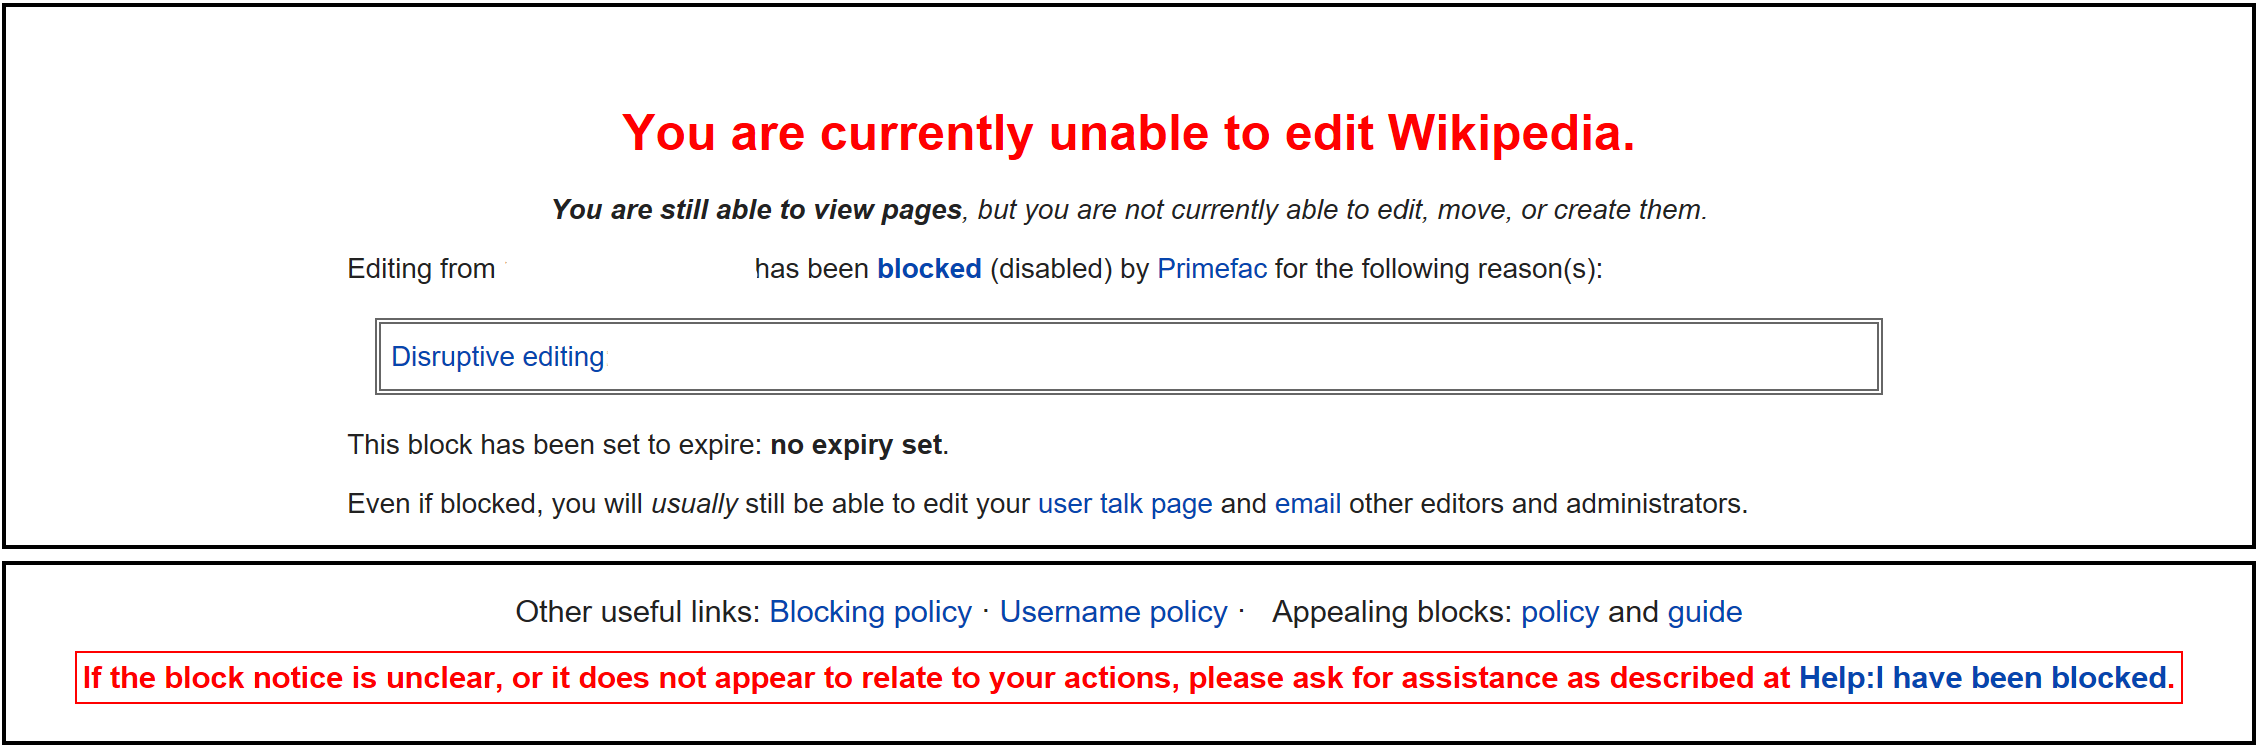
\includegraphics[width=\textwidth]{Blocknotice-wikipedia}
    \caption{A user's screen showing their ban from editing Wikipedia.}
  \end{minipage}
\end{figure}

However, a ban isn't strictly absolute because all the moderator does is ban a single online persona of a user -- a username. If it is relatively easy to join an online platform, then the user can always just make another account and continue on -- thus circumventing the ban. These alternate accounts are called \keyterm{sockpuppets} and are prevalent across online communities. This is one of the reasons that some online platforms are so susceptible to trolling -- since it is so easy to make another account, the offending user feels like they haven't really lost anything if they have been banned. Some online sites try to circumvent this by limiting a user's abilities until they have proven themselves. For example, Stack Overflow doesn't allow users to do anything except post and answer questions until they have earned enough "karma" points from being a good user of the site. Other online sites impose a time limit on when new user accounts can become active -- for example, a new account might not be able to interact with the site until 24 hours have passed. The hope is that offending users might become bored and lose interest in disrupting the site.

However, the downside of employing measures such as these is that it can turn off legitimate users, who might not want to start off with limited functionality or to wait some time before they can use the site. Thus, many sites opt not to employ these measures, leaving them susceptible to online trolls.

Some online platforms use a user's \keyterm{IP address} to try to prevent them from re-accessing their site. Every computer network is assigned a public IP address, which is a series of four numbers (at least in the IPv4 standard), which represents a user's computing network. If you want to find out your public IP address, you can simply type \texttt{what is my IP} in Google or visit \texttt{https://whatismyipaddress.com/}. Many homes have their own computing networks (so that you can access the Internet from home), each of which has its own public IP address. When you register a router with an Internet Service Provider (ISP), the ISP sends your router a public IP address, which your router shares with other devices on your computing network.

When a user sets up a sockpuppet account, it is likely from the same computer network (and probably the same computer!) that they ran the original account from. Thus, in order to combat sockpuppets, moderators can issue \keyterm{IP bans}, which ban an IP address rather than a user. IP bans are implemented similarly to regular bans; a separate blacklist is created which stores IP addresses and all IP addresses on the blacklist are prevented from accessing the online platform. If a user with a banned IP address tries to access the online platform, they will be prevented from doing so.

While IP bans have some effectiveness in combating sockpuppets, they also carry the possibility of banning innocent users who happen to belong to the same IP address as the offending user. For example, if someone in your household gets banned from an online gaming site and the online gaming site issues an IP ban, then you will be prevented from accessing the site as well even though you have done nothing wrong. This problem magnifies in cases of IP addresses which span multiple households or even entire communities. In one famous case from 2007, Wikipedia\index{Wikipedia} blocked an IP address based in Qatar from editing Wikipedia in response to "a large volume of spam and vandalism". The problem? That IP address covered the entirety of Qatar! Wikipedia ended up blocking the entire country of Qatar, over a million people, from editing Wikipedia [Arrington 2007].

Furthermore, while IP bans are often effective in deterring causal offenders, it is possible to get around IP bans. One important thing to note is that most IP addresses change and that they do so quite frequently. On average, a computer network will get a new IP address every nine months [Bojcic 2008]. Additionally, some ISPs issue a new IP address when a router is rebooted or when it is turned off and turned back on in the morning. Furthermore, while we won't go into specifics here, it is possible for a user to dodge an IP ban by changing the IP address their computer connects to the online platform from through the use of a \keyterm{VPN}, or virtual private network, such as NordVPN or ExpressVPN. A user can also connect indirectly to an online platform through a \keyterm{proxy server}, which it passes Internet traffic through to make it look like the user is connecting from the proxy server's IP address. If the user doesn't mind leaving their home, the user can also simply connect from another computer network -- perhaps from a local coffee shop or public library.

Sometimes we may not want to issue an IP ban because of the risk of unfairly banning innocent users who belong to the same IP address. Furthermore, since a dedicated user can get around an IP ban, IP bans also have limited effectiveness. One common strategy is to issue a \keyterm{shadow ban}. A moderator can shadow ban a user by taking away their ability to interact with other users without letting them know that they have lost this ability. A user won't know that they have been shadowbanned and will think they are still able to post or send messages to other users. However, other users won't receive their messages. The offending user won't be able to get a rise out of other users, who will seem to be ignoring him, causing the offending user to become bored of the social system and voluntarily leave.

TODO: Expand on shadowbanning

What if a user has been unfairly banned? Most large social systems have some sort of appeals process for users to plead their case if they believe they have been unfairly banned.

TODO: Expand on appeals process + give examples (e.g. Summoner Tribunal, moderator appeals).

\subsection{Content review}

How and when do moderators\index{moderation} review content? A social system might prevent content from being posted until it has been reviewed by a moderator. The benefit of this is that users can't see any content that hasn't been approved by a moderator. The downside of this is that this can introduce a long delay between when a user sends content and when other users can see the content. Thus, whether or not to use \keyterm{pre-approval}\index{pre-approval} is a trade-off between maintaining a safe environment and real-time posting. Many family-friendly online forums require all content to be pre-approved by a moderator because maintaining a safe environment is of paramount importance to them. Whereas on many discussion boards like Reddit\index{Reddit}, real-time posting is key and so pre-approval isn't used. To protect against trolls\index{troll}, sometimes discussion boards will require pre-approval on only the first five or ten posts that a user submits. This is enough to ward off most trolls while still allowing dedicated users to submit posts in real-time.

It is also common for social systems to allow users to \keyterm{flag}\index{flagging} content that they believe violates the rules of the social system. A moderator will then review the flagged content and issue a decision about it. Sometimes, the flagged content will be temporarily unavailable while the moderator reviews it. This method ensures that no-one else will view the flagged content, a benefit if the content is graphic or offensive. However, it is also frequently abused by trolls\index{troll} to harass users.

Unlike the pre-approval\index{pre-approval} method, the flagging\index{flagging} method is responsive rather than proactive. With pre-approval, no users view the content before it is reviewed, whereas, with flagging, many users might view the content before it is reviewed, and it might not ever be reviewed if it is not flagged.

\section{Volunteer moderation}

Process of applying to be a volunteer moderator

Expectations of volunteer moderators\\
 * Lower quality? Is it?

https://www.newyorker.com/tech/annals-of-technology/the-human-toll-of-protecting-the-internet-from-the-worst-of-humanity\\

Matias, Nathan J. "The Civil Labor of Online Moderators." In Internet Politics and Policy conference. Oxford, United Kingdom. 2016.\\
 * Many online platforms largely rely on volunteer moderators who are given limited administrative power to remove unacceptable content and ban problematic users.\\
 * Typically drawn from users most actively involved in community and invested in its success.

\section{Community moderation}

Sometimes communities self-moderate. They create \keyterm{blocklists}\index{blocklists}, which are lists of users who a community believe are toxic. They share these lists among other community members, who block the members on the lists. [Geiger 2016] Since these blocklists have no due process, many users on the blocklists feel that they have been unfairly blocked. [Jhaver et al. 2018]\index{moderation!self moderation}

TheBlockBot. 2016. The Block Bot. (2016). http://www.theblockbot.com\\
 * Block Bot emerged out of the use of hashtag \#BlockSaturday on Twitter. In 2012, a Twitter user began identifying accounts that he felt were worthy of blocking and started posting tweets containing the usernames of these accounts along with the \#BlockSaturday hashtag, so that his followers and anyone following the hashtag could block those accounts.

Hess, Amanda. 2014. "Twitter harassment: User-created apps Block Together, Flaminga, and the Block Bot crack down on Twitter abuse." (2014).\\
 * Block Bot expanded, allowing moderators to sort blocked users into three categories of offensiveness -- nasty, unpleasant and annoying, and allows subscribers to pick the level of offensiveness they would like to excise from their Twitter feeds.

Block Together

Good Game Auto Blocker (GGAB)

Donath, Judth S. 1999. Identity and deception in the virtual community. Communities in cyberspace 1996 (1999), 29-59.\\
 * Usenet employed "killfiles," filters that allowed Usenet users to skip unwanted postings. If a user put someone in their killfile, he stopped seeing any more of their postings. Found to be effective in keeping newsgroups readable. However, blocked users became resentful: "To the person who has been killed, Usenet becomes a corridor of frustratingly shut doors: one can shout, but cannot be heard."

\section{Psychological toll}

Henry Soto

Roberts, Sarah T. "Behind the screen: the hidden digital labor of commercial content moderation". Ph.D. Dissertation. University of Illinois at Urbana-Champaign. 2014.\\
 * Routine, factory-like nature of work of moderation leads to burnout among many workers.\\
 * Constant viewing of troubling content takes emotional toll on workers and they resist discussing their work with friends and family to avoid burdening them.

Kerr, Aphra and John D Kelleher. "The recruitment of passion and community in the service of capital: Community managers in the digital games industry." Critical Studies in Media Communication 32, 3 (2015) 177-192.\\
 * Many moderators have to perform emotional labor of enacting an "apolitical, culturally nuanced subjectivity" in their online work that may not align with their offline identity."

\section{Reading questions}
\begin{enumerate}
    \item What is the difference between commercial content moderation and self moderation?
    
    \item Facebook has come under fire for not removing graphic videos of shootings and suicides quickly enough. To solve this problem, in 2017, Mark Zuckerberg announced a plan to hire 3000 more moderators [Chaykowski 2017]. What downsides might result from this decision?
    
    \item Suppose a social media website decides to train a classifier to detect offensive language. The website uses Mechanical Turk to train the classifier, with the racial breakdown of workers being roughly 85\% white and 15\% African American. What problem might this classifier run into?
    
    \item A family-friendly MMO wants to better protect children by preventing them from typing their phone number in the chat. The MMO wants your advice on its proposals.
    \begin{enumerate}
        \item The MMO is thinking about implementing a blacklist and bans all numbers, both in numerical and word form. How might a user get around this blacklist?
        \item Heeding your advice, the MMO instead decides to implement a whitelist. The MMO whitelists all words in the Oxford English Dictionary except words meaning numbers. How might a user get around this whitelist?
        \item The MMO decides to continually expand its list of words which aren't allowed. Any word which users use to mean a number will be banned. Why is this approach problematic for the MMO?
    \end{enumerate}
\end{enumerate}

\section{Solutions to reading questions}
\begin{enumerate}
    \item Commercial content moderation is when a company hires moderators. Self moderation is when a community self-moderates.
    
    \item While removing graphic videos is certainly a good goal, commercial content moderators frequently face psychological harm in their job.
    
    \item Because of the disproportionate amount of white Mechanical Turk workers, the classifier might learn to flag African American Vernacular English. This will cause the algorithmic moderation to bias against African Americans.
    
    \item \begin{enumerate}
        \item The user could misspell the numbers (e.g. onne, twwo, thhree).
        \item The user could use words that look similar to numbers (e.g. won, too, tree).
        \item Removing all words that look similar to numbers will greatly disrupt normal chatting. Users will complain about the difficulty of use and become angry at the MMO.
    \end{enumerate}
\end{enumerate}

\section{Bibliography}

Arrington, Michael. "Wikipedia Bans Qatar." TechCrunch. January 1, 2007.

Bojcic, Dana. "How often do IP addresses change? (Example)" ViciMediaInc. May 2008.

Chandrasekharan, Eshwar et al. "You Can't Stay Here: The Efficacy of Reddit's 2015 Ban Examined Through Hate Speech." Proceedings of ACM Human-Computer Interaction. 1, 2, Article 31. November 2017.

Chaykowski, Kathleen. "Facebook Is Hiring 3,000 Moderators In Push To Curb Violent Videos." Forbes. May 3, 2017.

Chen, Adrian. "Inside Facebook's Outsourced Anti-Porn and Gore Brigade, Where 'Camel Toes' are More Offensive Than 'Crushed Heads'." Gawker. February 16, 2012.

Chen, Adrian. "When the Internets' Moderators are Anything But." The New York Times Magazine. July, 2015.

Crawford, Kate and Gillespie, Tarleton L. "What is a Flag for? Social Media Reporting Tools and the Vocabulary of Complaint." New Media \& Society. August, 2014.

Geiger, R. Stuart and Ribes, David. "The work of sustaining order in wikipedia: the banning of a vandal." Proceedings of the 2010 ACM conference on Computer supported cooperative work. pp. 117-126. 2010.

Geiger, R. Stuart. "Bot-Based Collective Blocklists in Twitter: The Counterpublic Moderation of Harassment in a Networked Public Space." Information, Communication, and Society 19(6). April 13, 2016.

Gillespie, Tarleton. "Governance of and by platforms." SAGE Handbook of Social Media. 2017.

Isaac, Mike. "Reddit Moderators Shut Down Parts of Site Over Employees Dismissal." The New York Times. July, 2015.

Jennings-Edquist, Grace. "What it's like being an online moderator (and how to make their lives easier)." ABC Life. September 10, 2019.

Jhaver, Shagun et al. "Online Harassment and Content Moderation: The Case of Blocklists." ACM Trans. Computer-Human Interaction. 25, 2, Article 1. March 2018.

Menking, Amanda and Erickson, Ingrid. "The Heart Work of Wikipedia: Gendered, Emotional Labor in the World's Largest Online Encyclopedia." Proceedings of the 33rd Annual ACM Conference on Human Factors in Computing Systems. pp. 207-210. 2015.

Newton, Casey. "The Trauma Floor: The secret lives of Facebook moderators in America." The Verge. February 25, 2019.

Popper, Ben. "YouTube CEO promises more moderation to prevent 'bad actors' from 'exploiting our openness'." The Verge. December 4, 2017.

Roberts, Sarah T. "Commercial Content Moderation: Digital Laborers' Dirty Work." Media Studies Publications. 12. 2016.

Seering, Joseph et al. "Shaping Pro and Anti-Social Behavior on Twitch Through Moderation and Example-Setting." Association for Computing Machinery 2017 Conference. 111-125. February 2017.

\textit{Sotos and Blauerts v. Microsoft}, (Florida Superior Court 2016).

\section{Image credits}

Picture of Wikipedia ban. By User:Awesome Aasim - Wikipedia, CC BY-SA 3.0, https://commons.wikimedia.org/w/index.php?curid=73734797

\end{document}
